%  cockshock2.tex - documentation source file

%  Written By - Philipp Klaus Krause

%  This program is free software; you can redistribute it and/or modify it
%  under the terms of the GNU General Public License as published by the
%  Free Software Foundation; either version 2, or (at your option) any
%  later version.

%  This program is distributed in the hope that it will be useful,
%  but WITHOUT ANY WARRANTY; without even the implied warranty of
%  MERCHANTABILITY or FITNESS FOR A PARTICULAR PURPOSE.  See the
%  GNU General Public License for more details.

%  You should have received a copy of the GNU General Public License
%  along with this program; if not, write to the Free Software
%  Foundation, 59 Temple Place - Suite 330, Boston, MA 02111-1307, USA.

%  In other words, you are welcome to use, share and improve this program.
%  You are forbidden to forbid anyone else to use, share and improve
%  what you give them.   Help stamp out software-hoarding!

\documentclass[a4paper]{article}
\usepackage{xltxtra}
\usepackage{siunitx}
\usepackage[pdftitle={cockshock2},pdfauthor={Philipp Klaus Krause}]{hyperref}

\begin{document}
\title{cockshock2}
\author{Philipp Klaus Krause}

\maketitle

\section{Introduction}

cockshock2 is an effort to reverse-engineer, document and hack a dog shock collar for use as an electrical torture device / sex toy.

It was inspired by the Master Series Cock Shock sex toy and it shortcomings (like the dog shock collars, it has an annoying auto shutdown timeout, but it also lacks adjustable intensity and is badly documented). There is another project on fixing the issues in the Cock Shock (https://github.com/spth/cockshock).

This project is based on a common dog-shock collar with adjustable intensity. The collar part is replaced by a shorter strip that better fits male genitals, the auto-shutdown timeout is disabled by replacing the tilt switch by a simple oscillator.

A long-term goal would be to replace the firmware with a free alternative.

\section{The Remote Control}

TODO: Description.

\begin{figure}
	\centerline{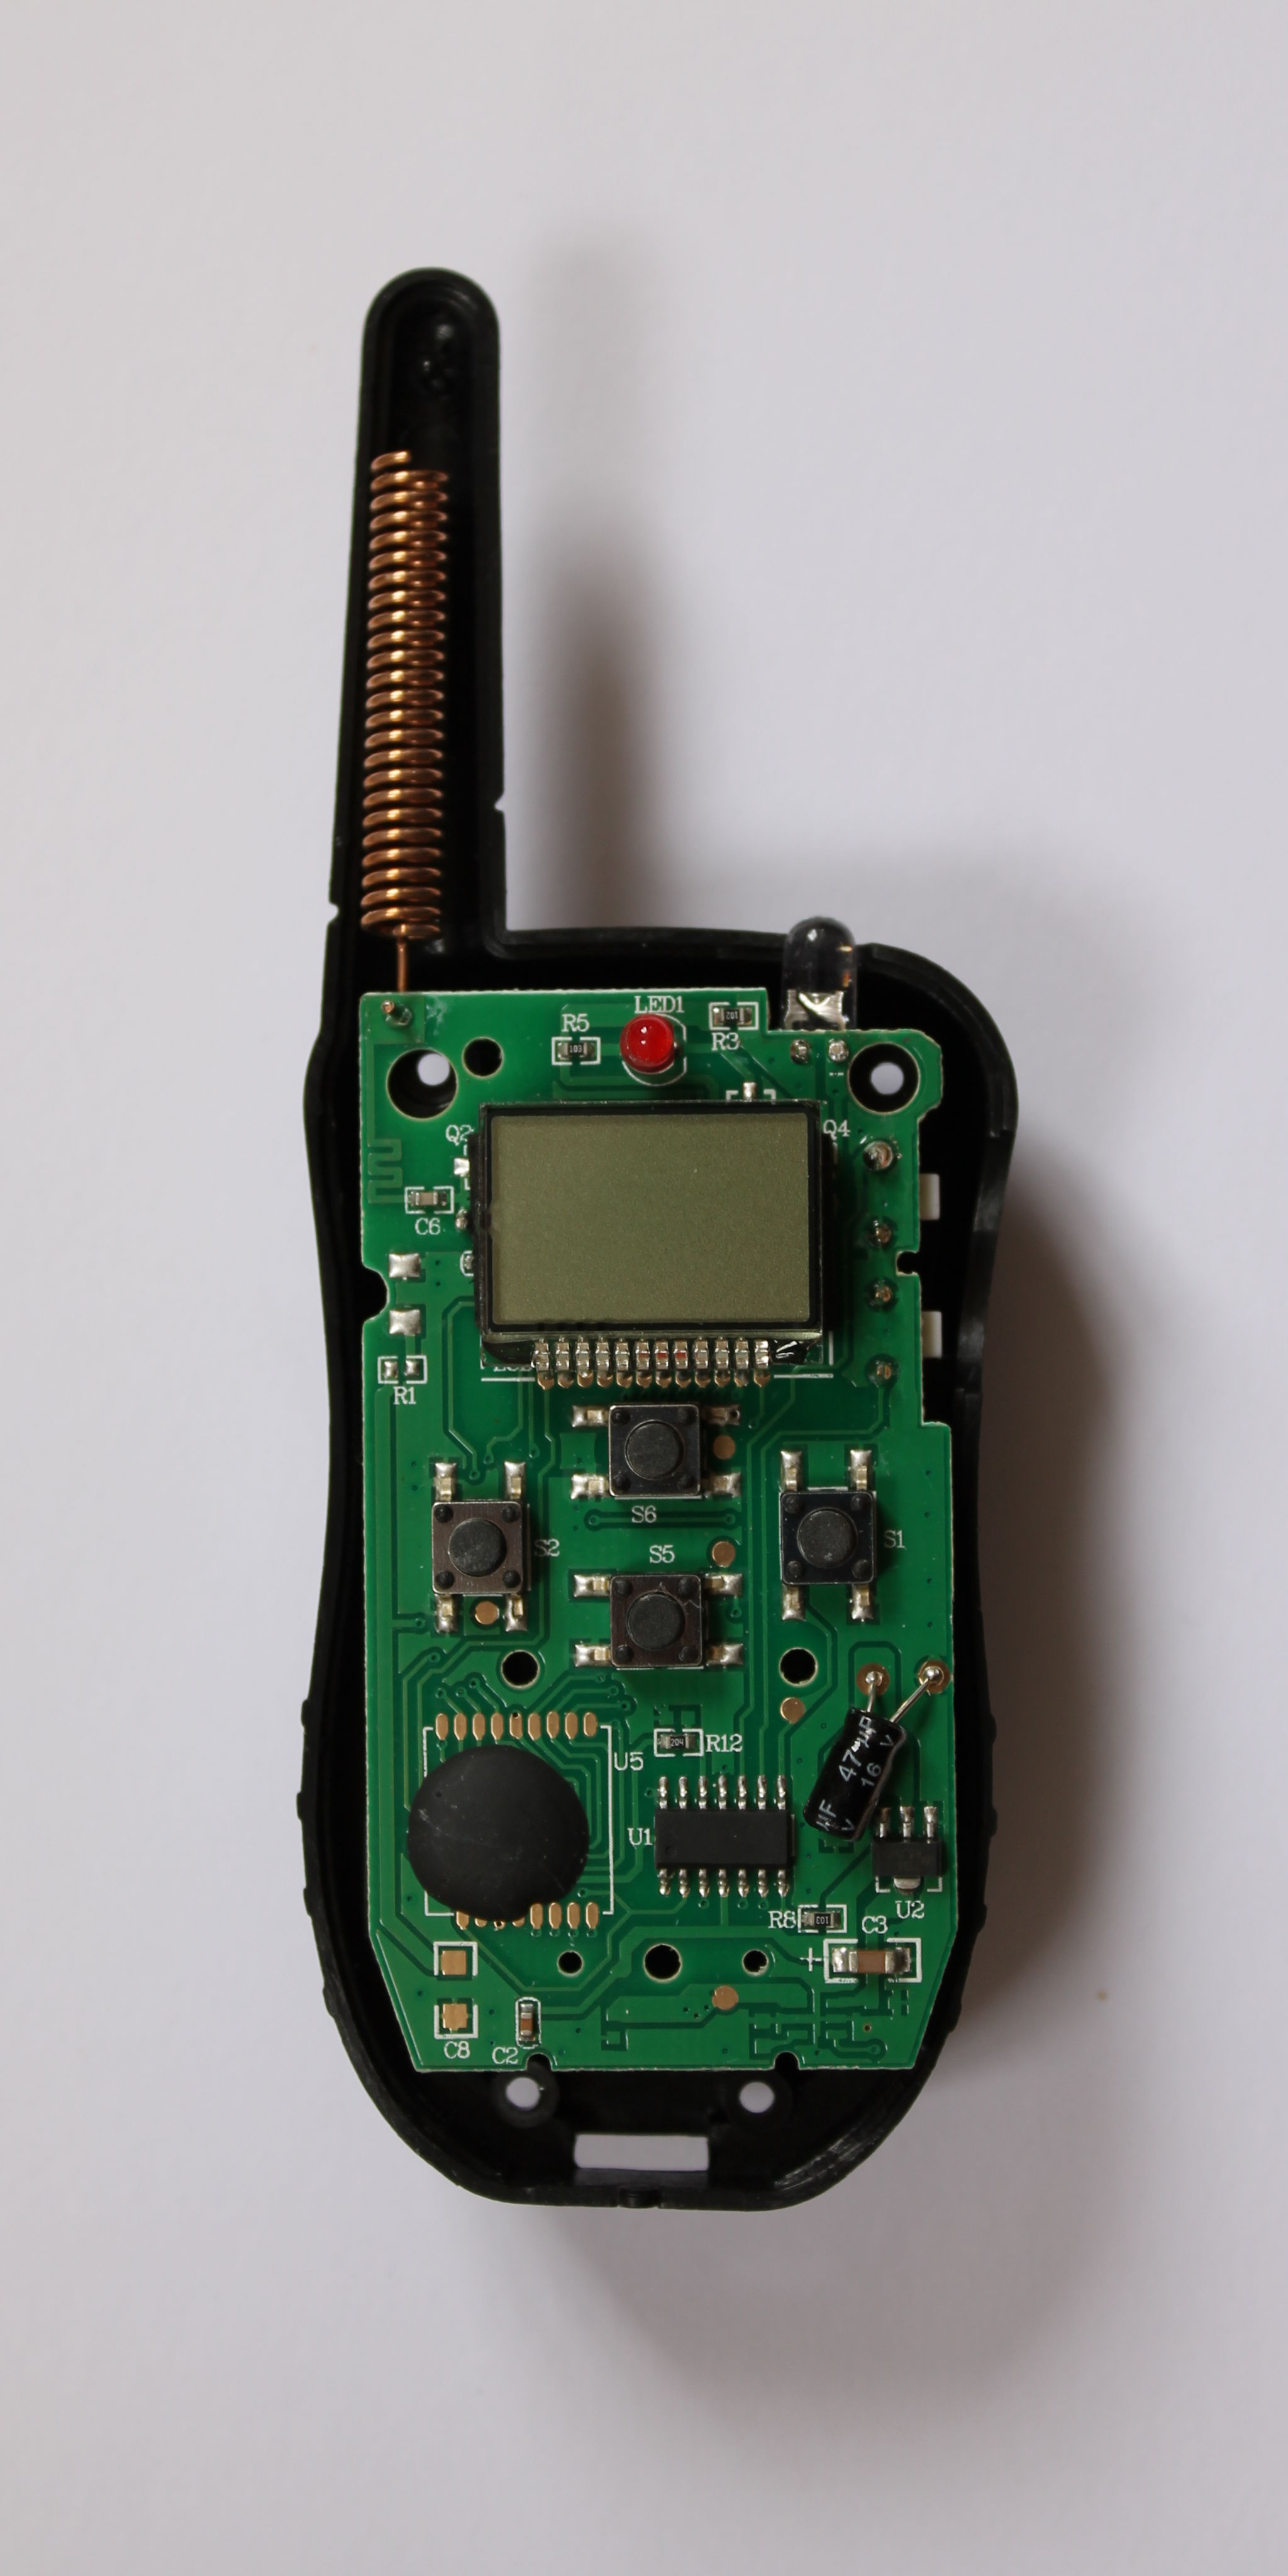
\includegraphics[scale=0.1]{remotecontrol-top.jpeg}}
	\caption{\label{remotepcb}Disassembled remote control}
\end{figure}

TODO: Schematics.

\section{The Shock Unit}

TODO: Description, schematics, document protoccol.

\section{Hack: Disable the 3-minute auto-shutdown timeout}

A simple modification is replacing the tilt switch in the shock unit by a slow (0.01 Hz to 10 Hz) Oscillator to disable the 3-minute auto-shutdown timeout.

\begin{figure}
	\centerline{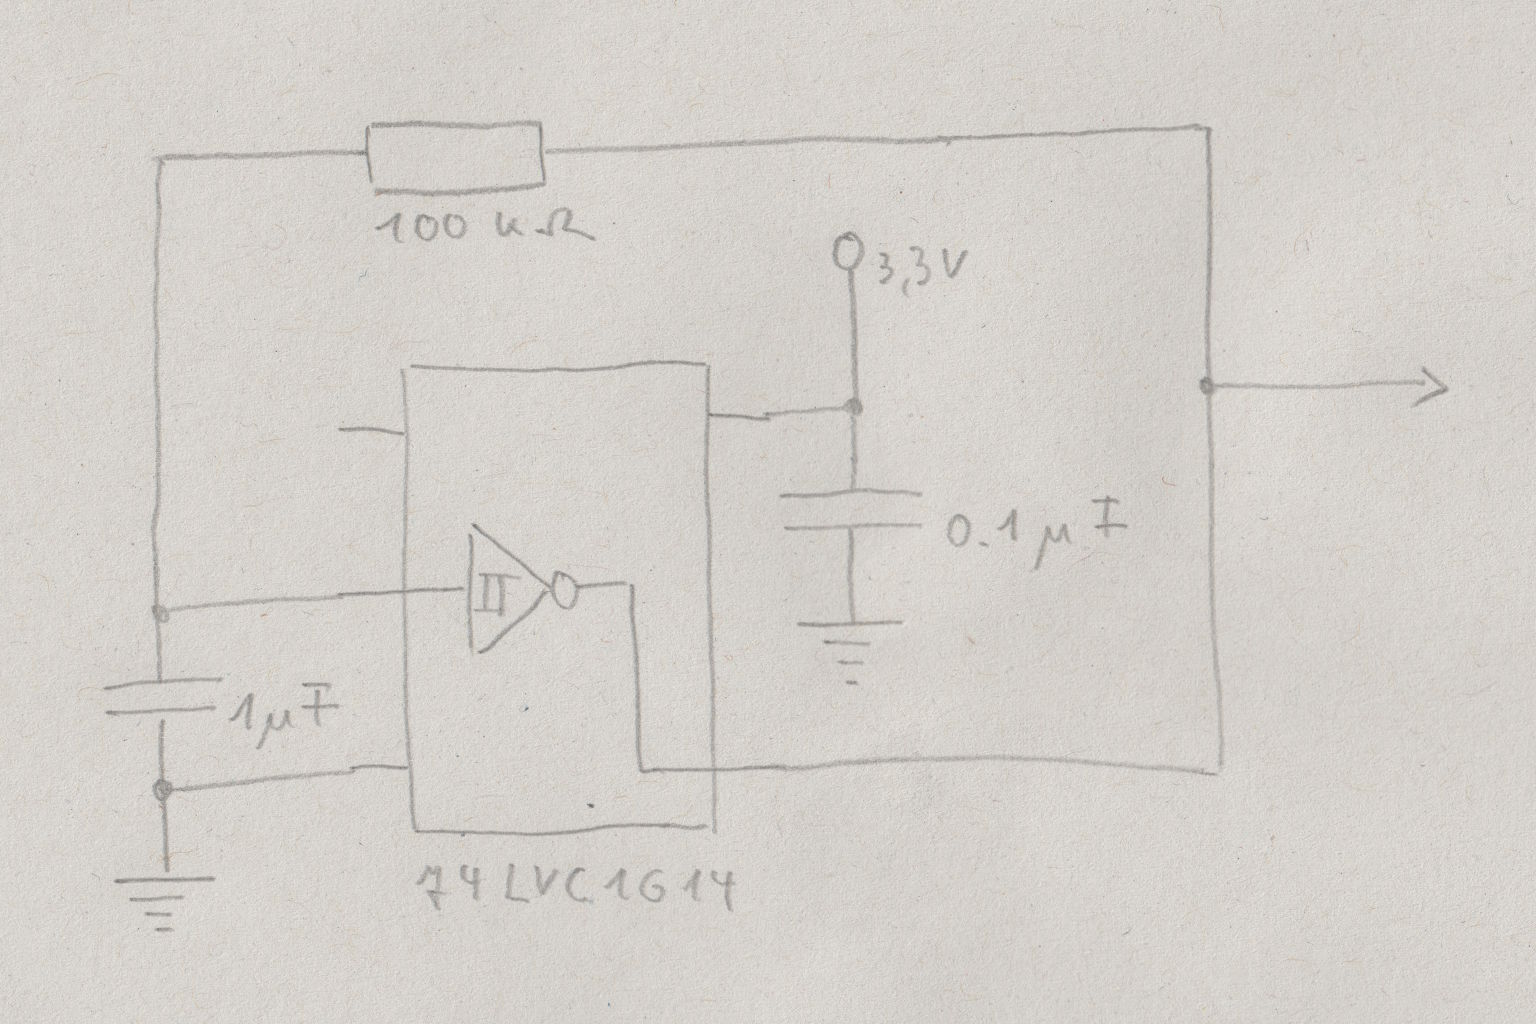
\includegraphics[scale=1.0]{auto-shutdown-timeout-hack.jpeg}}
	\caption{\label{auto-shutdown-timeout-hack}Oscillator for hack to disable auto-shutdown timeout}
\end{figure}

The oscillator can be built from just three small components: A 74LVC1G14 inverting Schmitt-trigger buffer, a 1 µF capacitor and a 100 k\si{\ohm} resistor (see Figure~\ref{auto-shutdown-timeout-hack}). Obviously, this hack increases power consumption; typical NiMH batteries will be drained in about two days, so after applying this hack the batteries should always be taken out of the shock unit when the shock unit is not used for a substantial time.

\end{document}

